\documentclass[border=10pt]{standalone}
\usepackage{tikz,amsmath}
\usetikzlibrary{arrows.meta}

% ========== 配色 ==========
\definecolor{hidFill}{RGB}{199,203,243}
\definecolor{hidLine}{RGB}{52,58,143}
\definecolor{inFill}{RGB}{183,224,177}       % 真实特征图绿色
\definecolor{inLine}{RGB}{32,102,32}
\definecolor{outFill}{RGB}{243,199,199}
\definecolor{outLine}{RGB}{143,52,52}
\definecolor{padFill}{RGB}{228,244,226}     % 浅浅绿色填充 (Padding)
\definecolor{padLine}{RGB}{120,170,120}     % padding 网格与虚线边框色 (柔和草绿)

\begin{document}
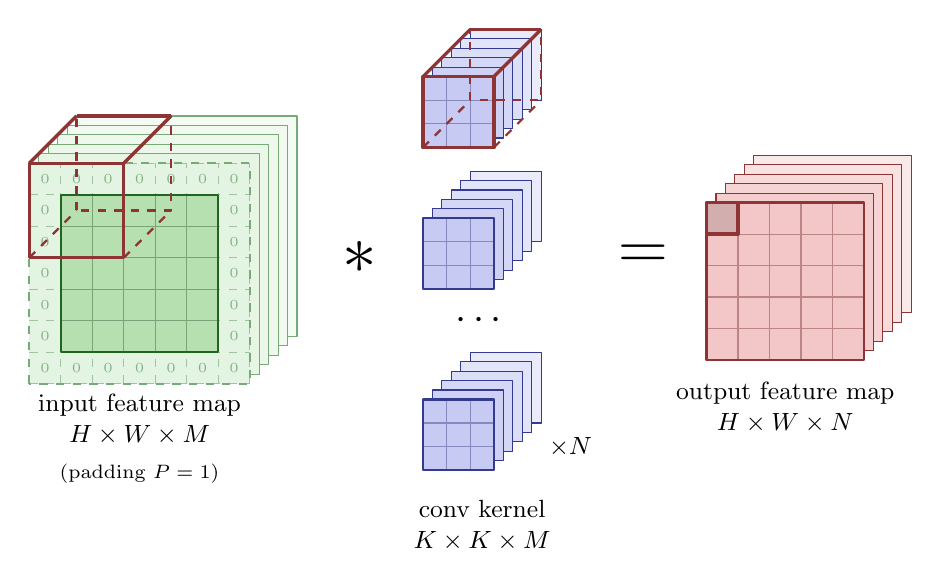
\begin{tikzpicture}[
    font=\small, line join=round,
    every node/.style={inner sep=0pt, outer sep=0pt, align=center}
  ]

  % ========== 普通堆叠宏 ==========
  % #1: x, #2: y, #3: 格数, #4: 每格尺寸, #5: 颜色前缀, #6: 背后叠加层数 (通道数 - 1)
  \newcommand{\stackbox}[6]{%
    \foreach \k in {#6,...,1}{%
      \pgfmathtruncatemacro{\op}{100-12*\k}
      \fill[#5Fill!\op, draw=#5Line, line width=.4pt]
            ({#1+0.12*\k},{#2+0.12*\k}) rectangle ++(#3*#4,#3*#4);
    }
    \fill[#5Fill] (#1,#2) rectangle ++(#3*#4,#3*#4);
    \draw[step=#4, #5Line!60, line width=.4pt, shift={(#1,#2)}] (0,0) grid (#3*#4,#3*#4);
    \draw[#5Line, thick] (#1,#2) rectangle ++(#3*#4,#3*#4);
  }

  % ========== 带 Padding 的堆叠宏 ==========
  % #1: x, #2: y, #3: 内层真实数据格数, #4: 每格尺寸, #5: 颜色前缀, #6: 通道数-1, #7: padding圈数
  \newcommand{\stackboxpad}[7]{%
    \pgfmathtruncatemacro{\totgrid}{#3 + 2*#7}
    \pgfmathsetmacro{\totdim}{\totgrid * #4}
    \pgfmathsetmacro{\indim}{#3 * #4}
    \pgfmathsetmacro{\padoff}{#7 * #4}
    % --- 背后叠加层 (通道深度从后往前绘制) ---
    \foreach \k in {#6,...,1}{%
      \pgfmathtruncatemacro{\op}{100-12*\k}
      % 背后 padding 浅浅绿色
      \fill[padFill!\op, draw=padLine, line width=.4pt]
            ({#1+0.12*\k},{#2+0.12*\k}) rectangle ++(\totdim,\totdim);
      % 背后 真实特征图区域
      \fill[#5Fill!\op, draw=#5Line, line width=.4pt]
            ({#1+0.12*\k+\padoff},{#2+0.12*\k+\padoff}) rectangle ++(\indim,\indim);
    }
    % --- 正面层 ---
    % 正面 padding 底色与虚线网格
    \fill[padFill] (#1,#2) rectangle ++(\totdim,\totdim);
    \draw[step=#4, padLine!70, dashed, line width=.4pt, shift={(#1,#2)}] (0,0) grid (\totdim,\totdim);
    % 正面 真实数据特征图底色与网格
    \fill[#5Fill] ({#1+\padoff},{#2+\padoff}) rectangle ++(\indim,\indim);
    \draw[step=#4, #5Line!60, line width=.4pt, shift={({#1+\padoff},{#2+\padoff})}] (0,0) grid (\indim,\indim);
    % 边框：特征图实线框，外圈 padding 虚线框
    \draw[#5Line, thick] ({#1+\padoff},{#2+\padoff}) rectangle ++(\indim,\indim);
    \draw[padLine, thick, dashed] (#1,#2) rectangle ++(\totdim,\totdim);
    % 正面 padding 单元格填入 0
    \pgfmathtruncatemacro{\lastidx}{\totgrid-1}
    \foreach \ix in {0,...,\lastidx}{%
      \node[font=\fontsize{5.5}{6.5}\selectfont, text=padLine!90] at ({#1+(\ix+0.5)*#4}, {#2+0.5*#4}) {0};
      \node[font=\fontsize{5.5}{6.5}\selectfont, text=padLine!90] at ({#1+(\ix+0.5)*#4}, {#2+(\lastidx+0.5)*#4}) {0};
    }
    \pgfmathtruncatemacro{\midend}{\lastidx-1}
    \foreach \iy in {1,...,\midend}{%
      \node[font=\fontsize{5.5}{6.5}\selectfont, text=padLine!90] at ({#1+0.5*#4}, {#2+(\iy+0.5)*#4}) {0};
      \node[font=\fontsize{5.5}{6.5}\selectfont, text=padLine!90] at ({#1+(\lastidx+0.5)*#4}, {#2+(\iy+0.5)*#4}) {0};
    }
  }

  % ========== 红色立体框宏 ==========
  \newcommand{\prism}[5]{%
    \draw[outLine, dashed, line width=.8pt]
          (#1+#5,#2+#5) rectangle (#1+#5+#3,#2+#5+#4);
    \draw[outLine, line width=1.2pt]
          (#1+#5,#2+#5+#4) -- (#1+#5+#3,#2+#5+#4);
    \draw[outLine, dashed, line width=.8pt]
          (#1,#2)--(#1+#5,#2+#5) (#1+#3,#2)--(#1+#3+#5,#2+#5);
    \draw[outLine, line width=1.2pt] (#1,#2) rectangle (#1+#3,#2+#4);
    \draw[outLine, line width=1.2pt]
          (#1,#2+#4)--(#1+#5,#2+#5+#4) (#1+#3,#2+#4)--(#1+#3+#5,#2+#5+#4);
  }

  % ========== 左：input 5x5 + 1层padding = 7x7 (6通道) ==========
  \stackboxpad{0}{0}{5}{.4}{in}{5}{1}
  \prism{0}{1.6}{1.2}{1.2}{0.6}
  \node at (1.4,-0.7) {input feature map\\$H\times W\times M$\\[2pt]\scriptsize(padding $P=1$)};

  % ========== 星号 ==========
  \node[font=\Huge] at (4.2,1.6) {$\ast$};

  % ========== 中：kernel 竖排一列 (6通道) ==========
  \stackbox{5.0}{3.0}{3}{.3}{hid}{5}
  \prism{5.0}{3.0}{0.9}{0.9}{0.6}

  \stackbox{5.0}{1.2}{3}{.3}{hid}{5}

  \node[font=\Large] at (5.75,0.8) {$\cdots$};
  \node[font=\small, anchor=west] at (6.6,-0.8) {$\times N$};

  \stackbox{5.0}{-1.1}{3}{.3}{hid}{5}
  \node at (5.75,-1.8) {conv kernel\\$K\times K\times M$};

  % ========== 等号 ==========
  \node[font=\Huge] at (7.8,1.6) {$=$};

  % ========== 右：output 5x5x6 (6通道) ==========
  \stackbox{8.6}{0.3}{5}{.4}{out}{5}
  \fill[outLine!40] (8.6,1.9) rectangle ++(0.4,0.4);
  \draw[outLine, line width=1.2pt] (8.6,1.9) rectangle ++(0.4,0.4);
  \node at (9.6,-0.3) {output feature map\\$H\times W\times N$};

\end{tikzpicture}
\end{document}